\section{Models}
\label{sec:models}

\begin{figure}[!htbp]
\centering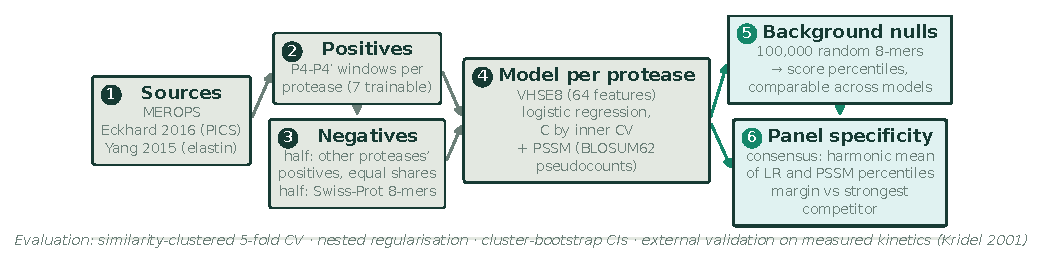
\includegraphics[width=\textwidth]{figures/F01_pipeline.pdf}
\caption{Overview of the pipeline from source data to panel selectivity.}
\label{fig:pipeline}
\end{figure}

\subsection{Physicochemical representation}
Each residue $a$ is mapped to $\varphi(a)\in\R^{8}$, its VHSE descriptor vector: eight principal-component score vectors derived by Mei et al.\ (2005) from independent families of $18$ hydrophobic, $17$ steric and $15$ electronic properties, of which VHSE1--2 are hydrophobic, VHSE3--4 steric and VHSE5--8 electronic. A window $w=(w_1,\dots,w_8)$ becomes
\begin{equation}
\bm{x}(w)=\bigl[\varphi(w_1);\,\varphi(w_2);\,\dots;\,\varphi(w_8)\bigr]\in\R^{64}.
\end{equation}
The descriptor table is archived with its source (\texttt{references/}) and unit-tested against it.

\paragraph{What this encoding can and cannot express.} A linear model on $\bm{x}$ has the additive form $\sum_i c_i^{\top}\varphi(w_i)$, so at each position the effect of the residue is a linear combination of the eight columns of the descriptor matrix $\Phi\in\R^{20\times8}$. Together with a constant, that confines each position's twenty-dimensional effect vector to a subspace of dimension $\operatorname{rank}[\Phi,\bm 1]=9$. A one-hot encoding has no such restriction ($19$ free parameters per position). Projecting each learned PSSM row onto the VHSE subspace shows that it captures $\subspaceMin$--$\subspaceMax\%$ of the variance of the position-specific log-odds, depending on the protease (Table~\ref{tab:controls}). The remaining variance is bias; the reduction from $19$ to $8$ parameters per position is the variance benefit. Section~\ref{sec:res-models} shows both sides of that trade-off empirically.

\subsection{Logistic regression}
\label{sec:lr}
Features are standardised using the training fold's means and standard deviations, $\bm z=(\bm x-\bm\mu)\oslash\bm\sigma$. The classifier minimises the class-weighted, L2-regularised logistic loss
\begin{equation}
\mathcal{L}(\bm\beta,b)=\tfrac12\|\bm\beta\|^2+C\sum_{i=1}^{n}\omega_{y_i}\log\bigl(1+e^{-\tilde y_i(\bm\beta^{\top}\bm z_i+b)}\bigr),\qquad \tilde y_i=2y_i-1,
\label{eq:lr}
\end{equation}
with ``balanced'' class weights $\omega_c=n/(2n_c)$, i.e.\ $\omega_1=2$ and $\omega_0=2/3$ at our $1{:}3$ ratio. The loss is strictly convex in $(\bm\beta,b)$ (its Hessian is $\bm I+C\sum_i\omega_{y_i}p_i(1-p_i)\tilde{\bm z}_i\tilde{\bm z}_i^{\top}\succ0$ with $\tilde{\bm z}=[\bm z;1]$ apart from the unpenalised intercept), so the optimiser (L-BFGS) finds the unique minimum. The regularisation strength $C\in\{10^{-3},\dots,10^{2}\}$ is chosen by an inner cross-validation on the training data only (Section~\ref{sec:cv}).

\begin{derivation}[Meaning of the balanced weights]
Equal total weight on the two classes is equivalent to fitting the posterior under a $50{:}50$ prior. If $\rho=p_{\mathrm{bal}}/(1-p_{\mathrm{bal}})$ is the fitted odds, the odds under the actual $1{:}3$ training mixture are $\rho/3$, so $p_{\mathrm{mix}}=p_{\mathrm{bal}}/(3-2p_{\mathrm{bal}})$. Neither is the probability that a random window is cleaved, which is far smaller. This is why the reliability curves in Figure~\ref{fig:calib} lie away from the diagonal and why we never present the score as a probability.
\end{derivation}

\paragraph{Per-position decomposition.} Because the logit is linear in $\bm z$, it splits exactly into one term per position,
\begin{equation}
\mathrm{logit}(w)=b+\sum_{i=1}^{8}\kappa_i(w),\qquad \kappa_i(w)=\sum_{d=1}^{8}\beta_{id}\,z_{id}(w),
\label{eq:decomp}
\end{equation}
which the interactive tool draws as a bar per position.

\subsection{Position-specific scoring matrix}
For observed residue counts $n_{i}(a)$ among $n$ positives, let $f_i(a)=n_i(a)/n$. Rare residues are smoothed toward a substitution-weighted expectation. Let $W$ be the row-normalised positive part of BLOSUM62, $W_{ab}\propto\max(S_{ab},0)$, and $q_i=f_i W$; mix in the Swiss-Prot background $g$ so that no residue has zero probability:
\begin{equation}
Q_i=(1-\epsilon)\,q_i+\epsilon\,g,\qquad p_i(a)=\frac{n\,f_i(a)+\beta\,Q_i(a)}{n+\beta},\qquad S(w)=\sum_{i=1}^{8}\log_2\frac{p_i(w_i)}{g(w_i)},
\label{eq:pssm}
\end{equation}
with $\beta=5$ pseudo-observations and $\epsilon=0.05$. This is a heuristic pseudocount scheme, not the block-based estimator that BLOSUM62 itself derives from; it is fully specified and unit-tested, and it has no fitted hyperparameter beyond $\beta,\epsilon$. Position $i$ carries $\mathrm{IC}_i=\sum_a p_i(a)\log_2\!\bigl(p_i(a)/g(a)\bigr)$ bits, which sets the letter heights in Figure~\ref{fig:logos}.

\subsection{Background null, percentiles and panel selectivity}
\label{sec:null}
\paragraph{Why raw scores cannot be compared.} Different proteases are trained on different positives and different negatives, so their logits and PSSM scores live on different scales. Even the average LR score on a random window differs by model (Figure~\ref{fig:calib}b), which makes a ratio such as $p_t/\max_{j\ne t}p_j$ depend on the training set of each model rather than on the peptide.

\paragraph{Percentile transform.} For protease $k$ and score $s_k$, let $F_k$ be the distribution function of $s_k(W)$ over random windows $W$ drawn from the background composition. We report $u_k^{\mathrm{LR}}(w)=F_k^{\mathrm{LR}}(s_k^{\mathrm{LR}}(w))$ and $u_k^{\mathrm{PSSM}}(w)=F_k^{\mathrm{PSSM}}(s_k^{\mathrm{PSSM}}(w))$. By the probability integral transform, each is uniform on $[0,1]$ under the null for every protease, so values are directly comparable across models (Appendix~\ref{app:deriv}); each is also invariant to any monotone rescaling of its score. $F_k$ is estimated from $100{,}000$ random windows and stored as a $1{,}001$-point quantile grid, interpolated linearly, so the resolution at the top of the range is $10^{-3}$.

\paragraph{Consensus and margin.} The two percentiles are combined by their harmonic mean,
\begin{equation}
u_k(w)=\frac{2\,u_k^{\mathrm{LR}}(w)\,u_k^{\mathrm{PSSM}}(w)}{u_k^{\mathrm{LR}}(w)+u_k^{\mathrm{PSSM}}(w)},
\label{eq:cons}
\end{equation}
which is high only when both scorers agree. For a target $t$ in a panel $\mathcal{P}$, the specificity margin is
\begin{equation}
M_t(w;\mathcal{P})=u_t(w)-\max_{j\in\mathcal{P}\setminus\{t\}}u_j(w)\ \in[-1,1].
\label{eq:margin}
\end{equation}
A margin near $+1$ means the window is in the extreme tail for the target and near the bulk for every competitor; a margin near $0$ means it is as strongly recognised by some competitor as by the target. The margin depends on the panel by construction.

\subsection{Windows with unknown positions}
Sensor cores are often shorter than eight residues around the bond, so some positions are unknown (marked ``$-$''). Both scorers are additive over positions, which gives a principled treatment. For the logit, an unknown position contributes its training mean, $z_{id}=0$, which equals the expectation of the linear score under any distribution of that feature with the training mean. For the PSSM, an unknown position contributes the background expectation $\sum_a g(a)\log_2(p_i(a)/g(a))$. Percentiles are then taken against a null computed with the \emph{same} positions masked, so that a gapped window is compared with equally uninformed random windows.

\subsection{Portability}
Each trained model is a plain JSON file of arrays (feature means and scales, coefficients, intercept, the $8\times20$ PSSM, and the two quantile grids). The Python package and the browser tool read the same files and are tested for numerical agreement.
